\section{Unity Physik}
\label{sec:physik}
Unitys eingebaute Physik-Engine ermöglicht die realistische Berechnung von Kollisionen, Schwerkraft und anderen Kräften, was Entwicklern hilft, immersive und interaktive Umgebungen zu schaffen.

Die Festkörperkomponente (Rigidbody) erlaubt es, 3D-Objekte als nicht verformbare Einheiten innerhalb dieses Systems zu simulieren. Dies ist entscheidend für die Entwicklung realistischer physikalischer Interaktionen, wie z. B. das Bewegen von Objekten, die auf Kräfte, Drehmomente und Kollisionen reagieren.

\begin{figure}[H]
  \centering  
  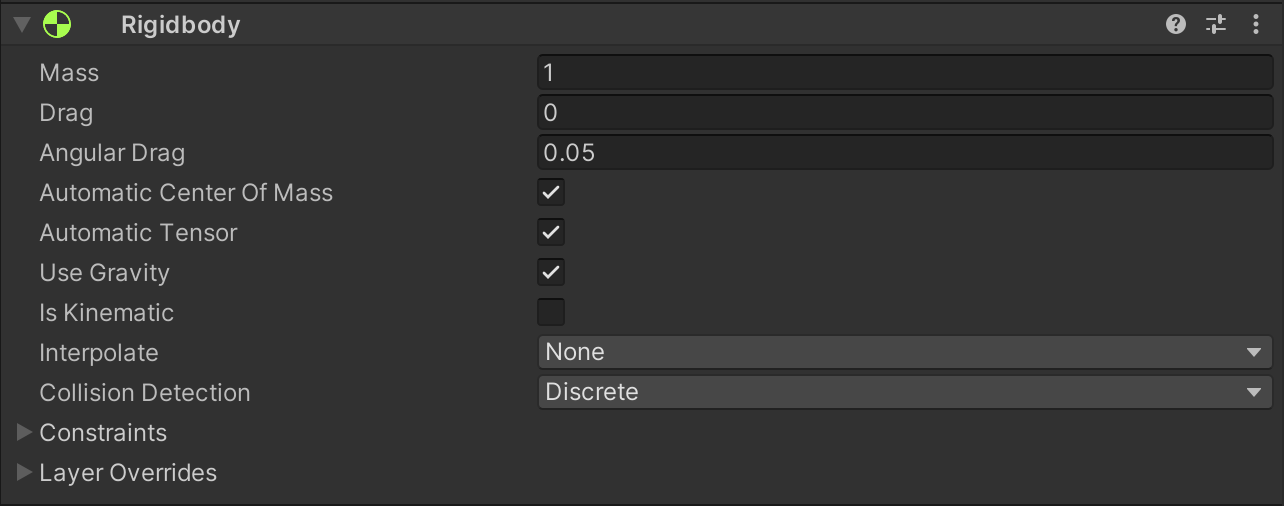
\includegraphics[scale=0.5]{img/physik_festkoerper.png}
  \caption{Unity ML-Agents Physik Festkörper}
  \label{fig:physik_festkoerper}
\end{figure}
\begin{itemize}
  \item Mass: gibt das Gewicht des Körpers an
  \item Drag: definiert den Geschwindigkeitsverlust eines Körpers in Bewegung durch Reibung, Luftwiederstand
  \item Angular Drag: definiert den Geschwindigkeitsverlust eines Körpers für Rotationsbewegung
  \item Collision Detection: legt fest wie Kollisionen berechnet werden (Akkurat/Leistung)
 \end{itemize}
 
Um Kollisionen zwischen Objekten zu berechnen benötigen diese zusätzlich eine Kollisionskomponente. Komplexe 3D-Modelle können in der Kollisionsberechnung jedoch in ihrer direkten Form rechenintensiv sein. Zur Optimierung werden diese Modelle vereinfacht, indem sie durch geometrische Formen wie Kugeln, Kapseln oder Boxen dargestellt werden. Abbildung \ref{fig:physik_kollision} zeigt die Unterschiedlichen Kollisionskomponenten in Unity. Abbildung \ref{fig:physik_kollision_charakter} zeigt wie die Kollisionkomponenten (gelbe Wireframes) genutzt werden um die Körperteile eines komplexen 3D Modells vereinfacht abzubilden.

 \begin{figure}[H]
  \centering  
  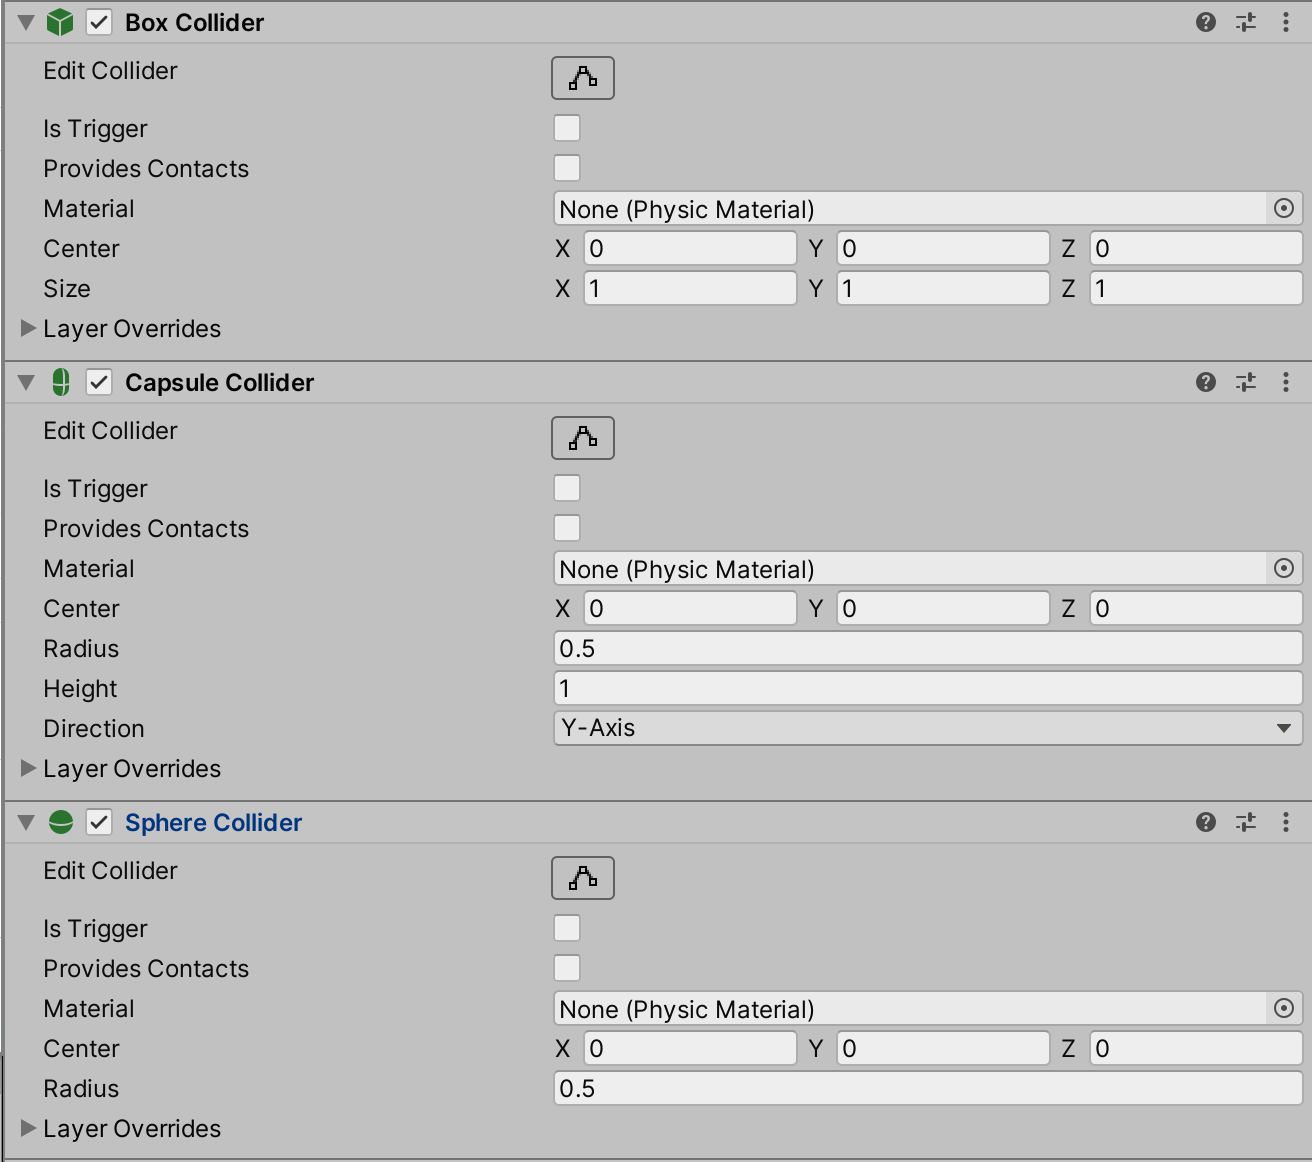
\includegraphics[scale=0.5]{img/physik_kollision.png}
  \caption{Unity ML-Agents Physik Kollisionskomponenten}
  \label{fig:physik_kollision}
\end{figure}

 \begin{figure}[H]
  \centering  
  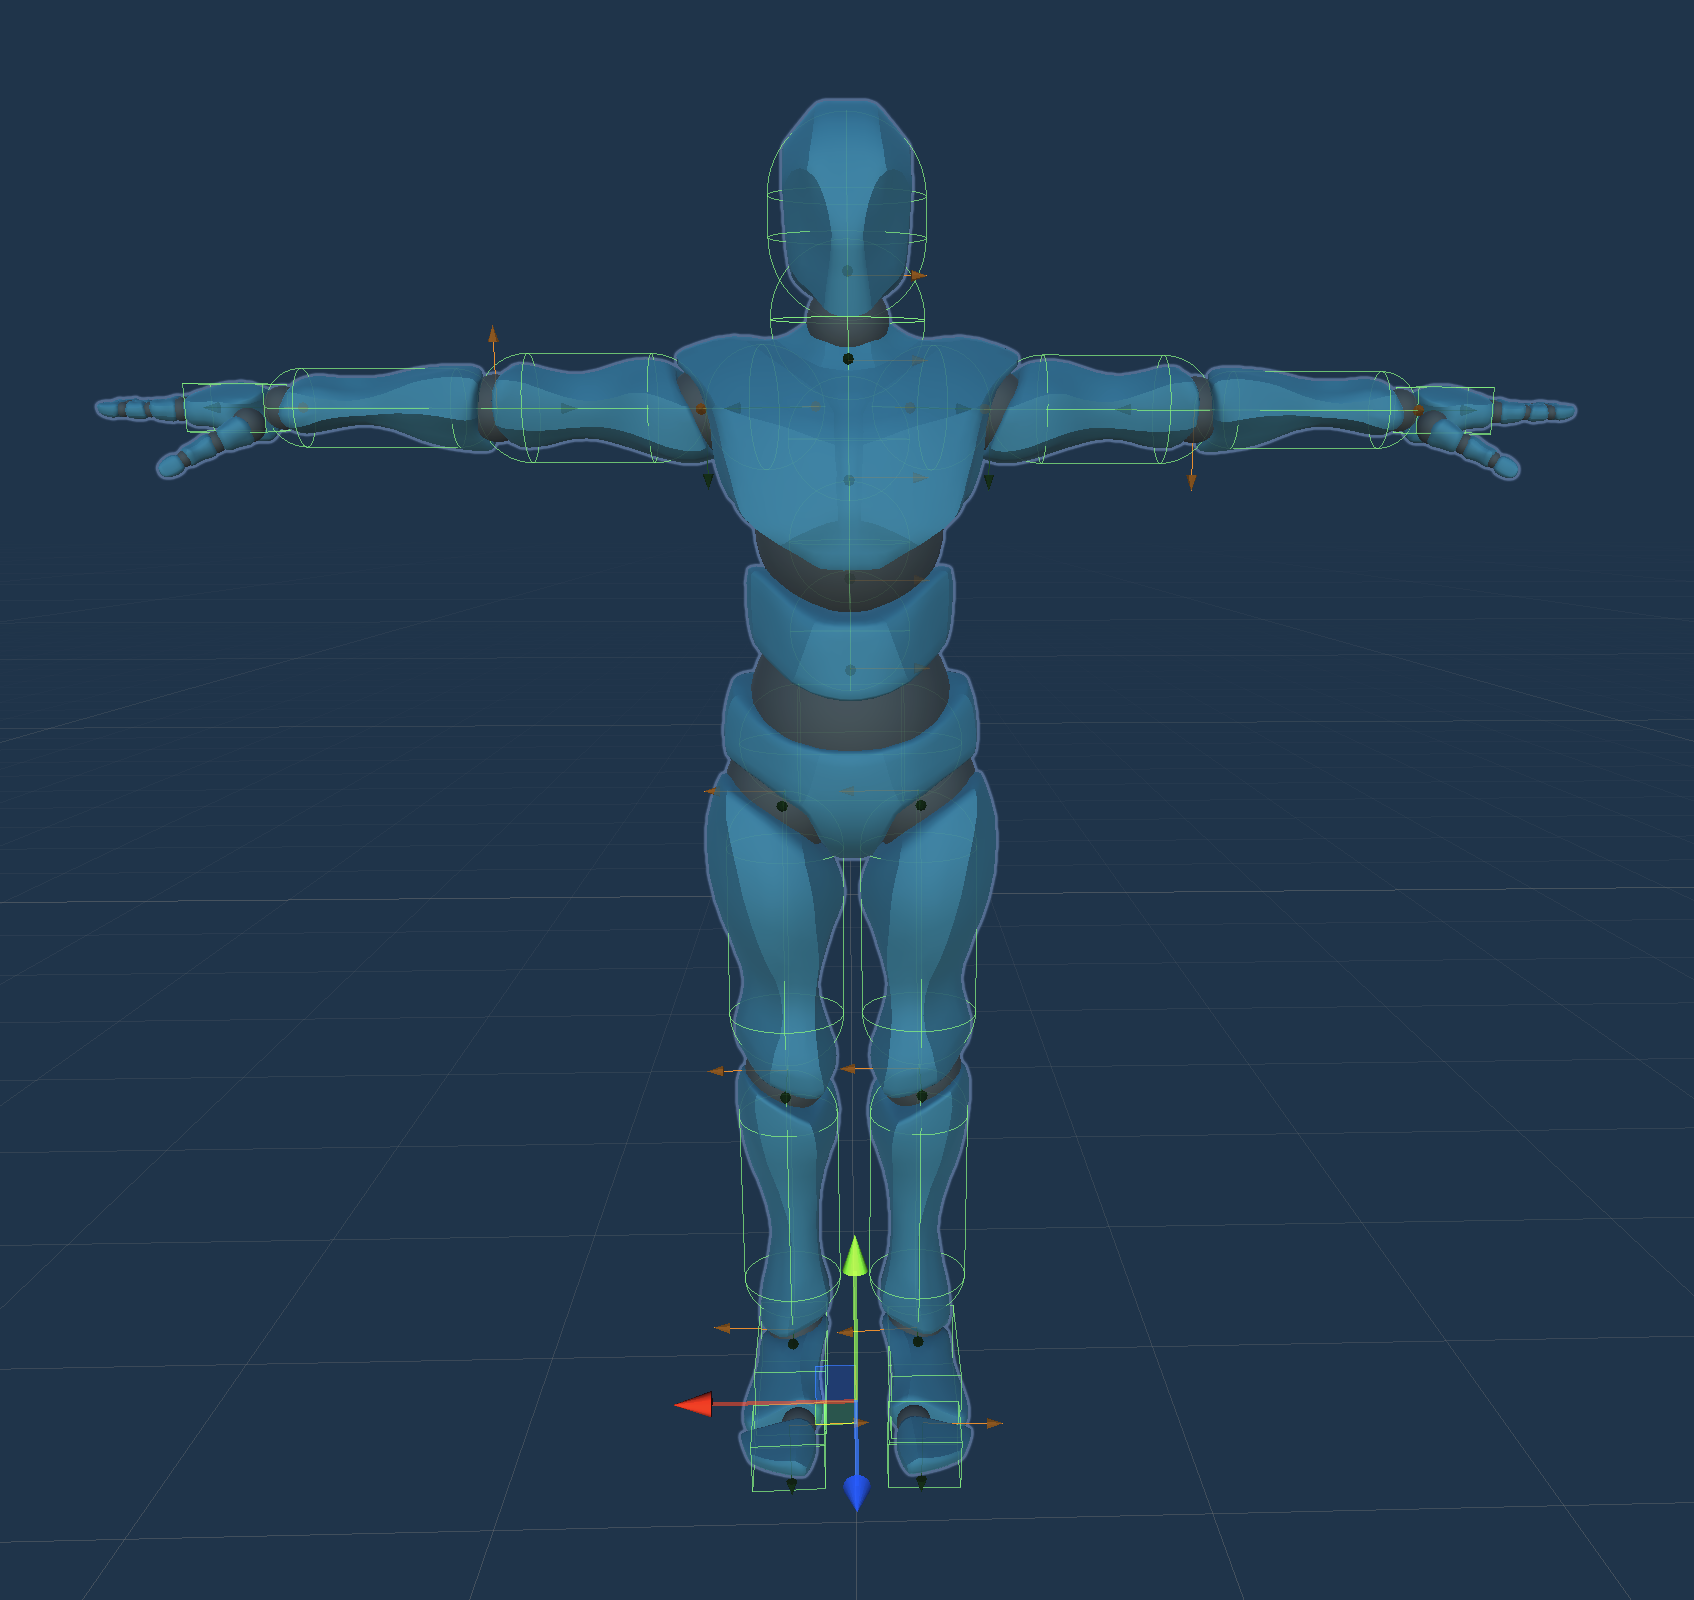
\includegraphics[scale=0.5]{img/physik_kollision_charakter.png}
  \caption{Unity ML-Agents Physik Charakter vereinfacht mit Kollisionskomponenten }
  \label{fig:physik_kollision_charakter}
\end{figure}

Festkörper können mit Gelenken zu komplexeren Körperstrukturen verbunden werden. Die Konfigurierbare Gelenkkomponente (Configurable Joint) ermöglicht die Simulation von Gelenken mit freier Bewegung und Rotation auf allen drei Achsen. Dies ist wesentlich, um realistische Animationen und Interaktionen in Softwaresimulationen zu erzeugen. Im Kontext dieser Arbeit wird das Gelenk auf Rotation beschränkt und als kugelförmiges Gelenk verwendet. Die Gelenke einer humanoiden Figur können somit vereinfacht aber ausreichend genau simuliert werden.

\begin{figure}[H]
  \centering
  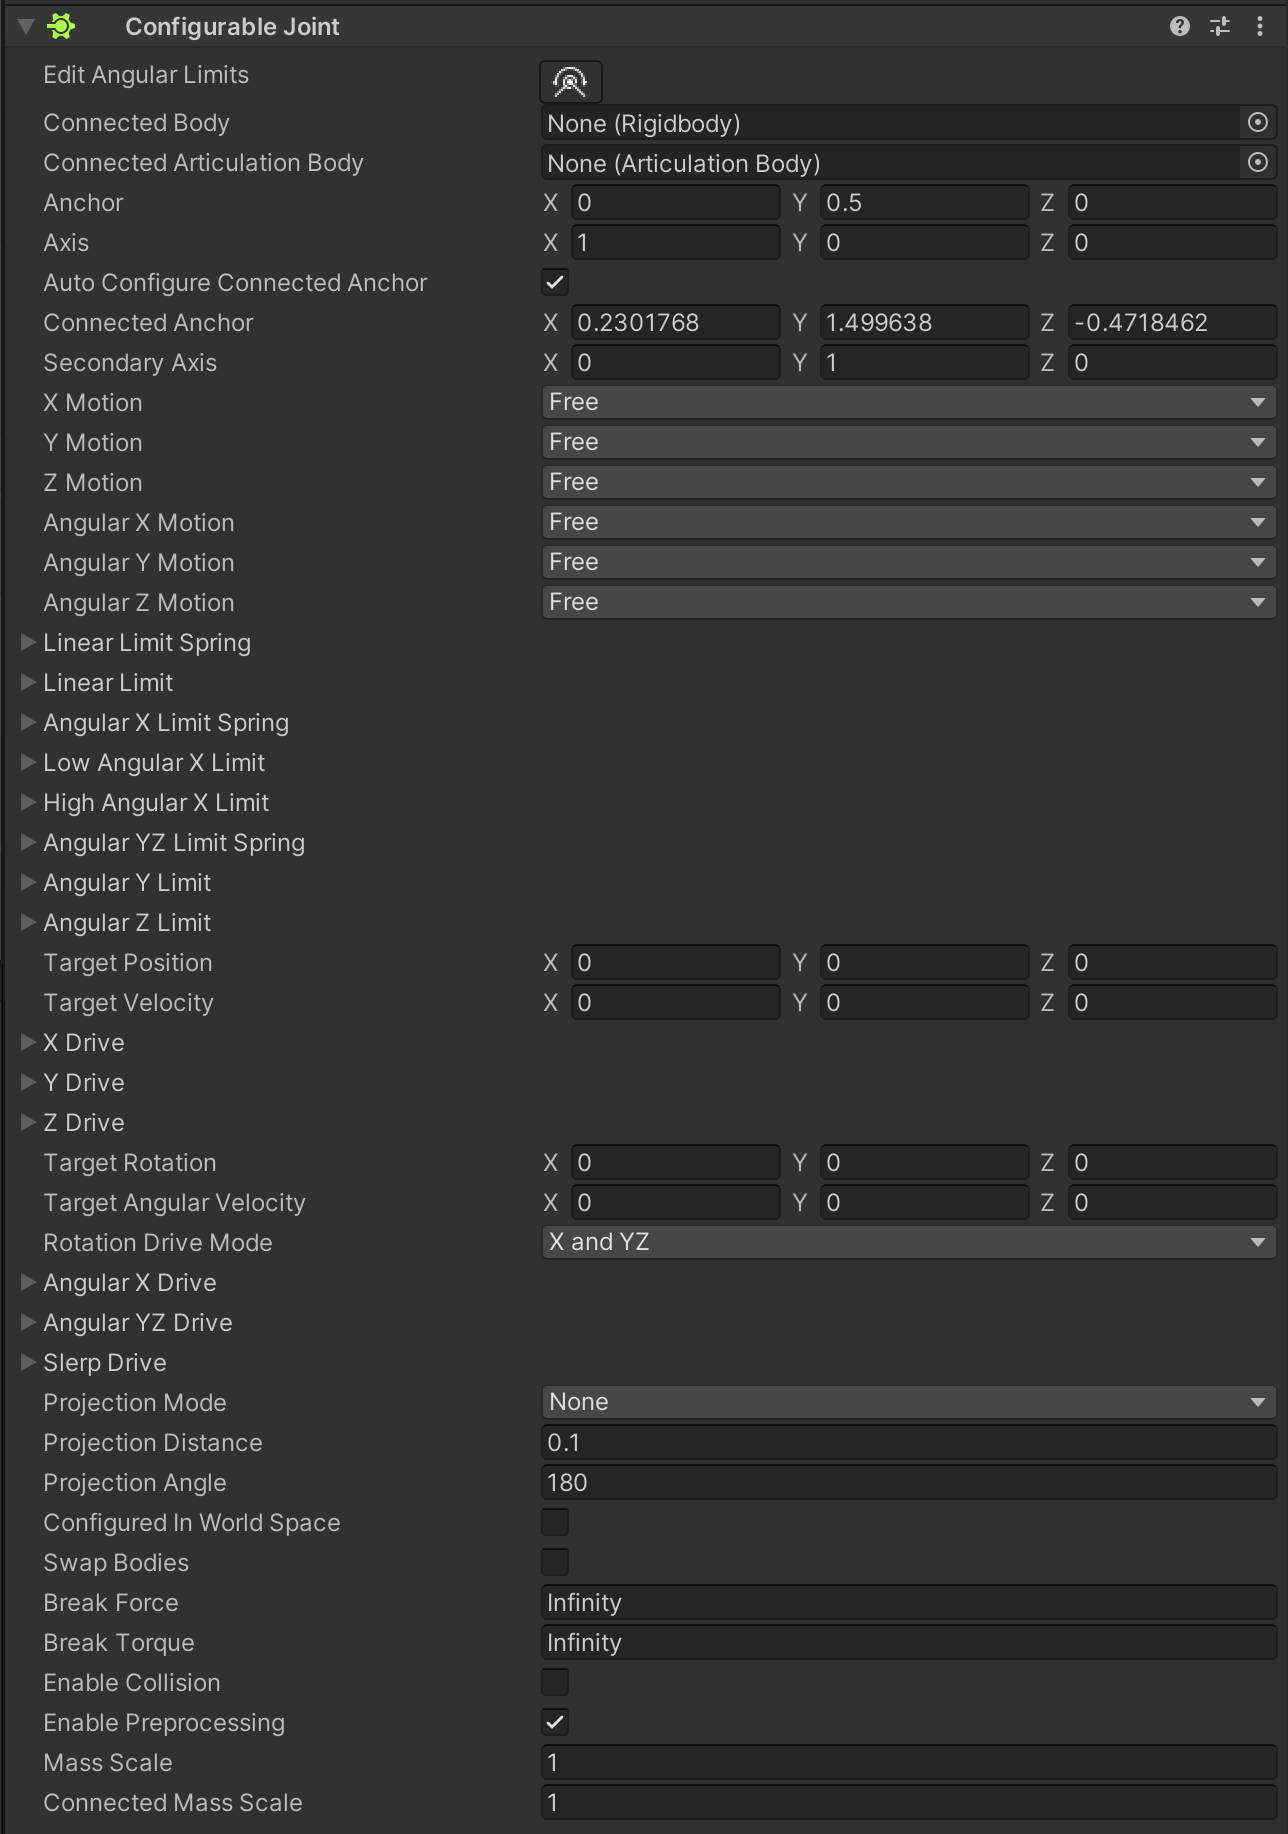
\includegraphics[scale=0.5]{img/physik_gelenk.png}
  \caption{Unity ML-Agents Physik Gelenk}
  \label{fig:physik_gelenk}
\end{figure}
\begin{itemize}
  \item Connected Body: bestimmt, mit welchem Körper das Gelenke verbunden ist
  \item Anchor: legt fest, an welchem Punkt die Verbindung zum verbundenen Körper besteht
  \item Axis: legt die Hauptbewegungs- und Rotationsachse fest
  \item Secondary Axis: legt die sekundäre Beweungs- und Rotationsachse fest
  \item Angular X Y Z Motion: bestimmt, ob das Gelenk Rotation zwischen den Körpern auf der X Y Z Achse zulässt
  \item Target Position: bestimmt das Ziel, zu welchem das Gelenk sich bewegen soll
  \item Angular X Y Z Limit: ermöglicht das Festlegen von Winkellimits für die Rotationsbewegungen
  \item X Y Z  und Slerp Drive: bestimmen die Stärke der Federkraft welche das Gelenk in die Zielposition bewegt
\end{itemize}